\chapter{Produtos, Atividades e Cronograma}

\section{Resumo da Proposta}
	O processo de medição será realizado sobre o objeto da disciplina de Introdução a Jogos Eletrônicos. Neste objeto serão realizados processos de medição no contexto do produto e da equipe de desenvolvimento. O processo de medição será iniciado juntamente com o desenvolvimento do projeto, podendo dessa forma auxiliar ativamente a equipe a melhorar seu processos administrativos e de desenvolvimento.
	
	A medição será iniciada com o levantamento dos objetivos de negócio, que representam as metas buscadas pela equipe no desenvolvimento do jogo. Com os objetivos definidos serão levantadas questões que auxiliarão na descoberta de elementos, métricas, que podem ajudar a concretizar os objetivos estabelecidos.

	A avaliação da disciplina de Introdução aos Jogos Eletrônicos será avaliada em marcos, indicando também quando serão coletados os dados relacionados a medição do processo de desenvolvimento, sendo eles:

	\begin{itemize}
		\item Marco 1: 19/04 (Esse marco não será medido, pois será apenas apresentação da ideia do jogo)
		\item Marco 2: 05/05/2017
		\item Marco 3: 31/05/2017
		\item Marco 4: 21/06/2017
		\item Marco 5: 07/07/2017 - Apresentação do jogo completo
	\end{itemize}

\newpage

\section{Estrutura Analítica do Projeto}
	\begin{figure}[!htpb]
		\centering
		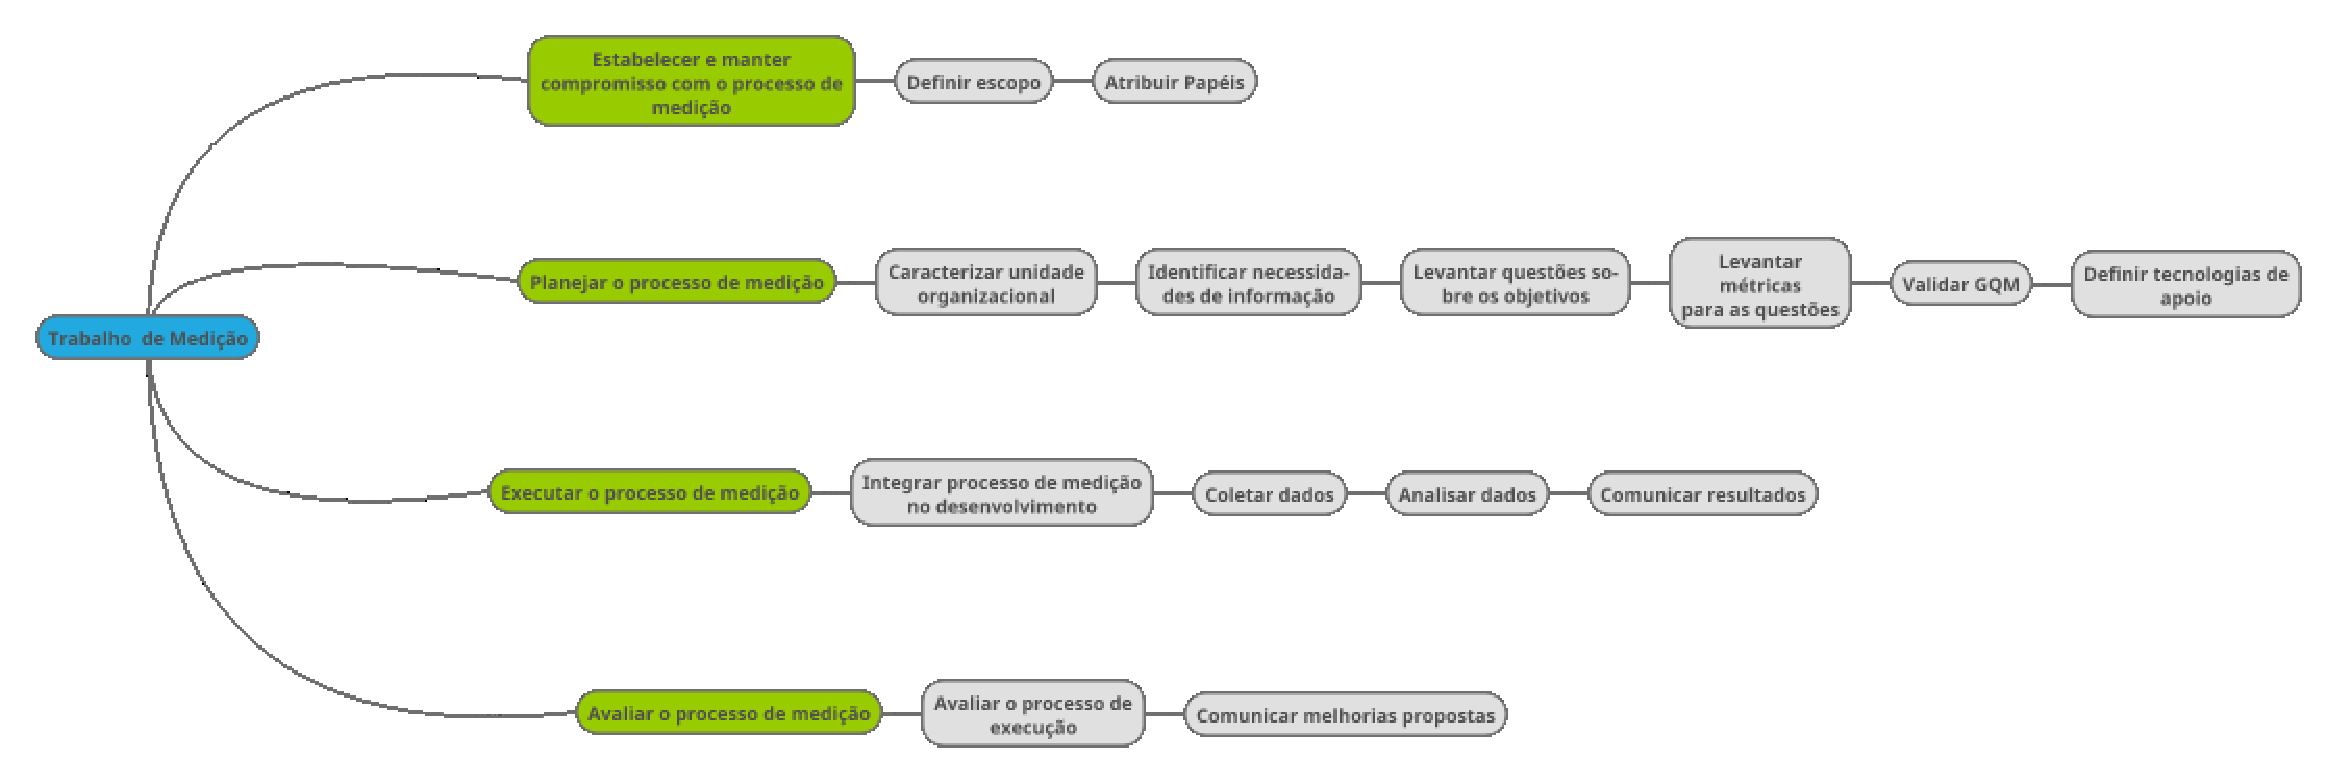
\includegraphics [scale=0.42]{figuras/processo/eap}
		\caption{Estrutura Analítica do Projeto}
	\end{figure}
	
\section{Lista de Software}
	As ferramentas necessárias para o desenvolvimento do produto de software da disciplina de Introdução a Jogos Digitais serão: 
	\begin{itemize}
		\item Ferramenta de Gerenciamento de Versão Git
		\item Linguagem C++ e biblioteca SDL
	\end{itemize}
	
	As ferramentas utilizadas pela equipe de medição para auxiliar na coleta de métricas e para produção da documentação serão:
	
	\begin{itemize}
		\item Draw.io para produção dos modelos de processo e diagramas
		\item Simian e cLint para coleta de métricas relacionadas ao desenvolvimento do software (código)
		\item Wakatime para coleta de métricas relacionadas a tempo
	\end{itemize}
	
\section{Cronograma}
	O cronograma foi utilizado para organizar os processos da primeira e da segunda entrega relacionados ao projeto de medição em formato sequencial, bem como definir quais os integrantes participarão de cada atividade e o tempo de duração das mesmas.
	\begin{figure}[!htpb]
		\centering
		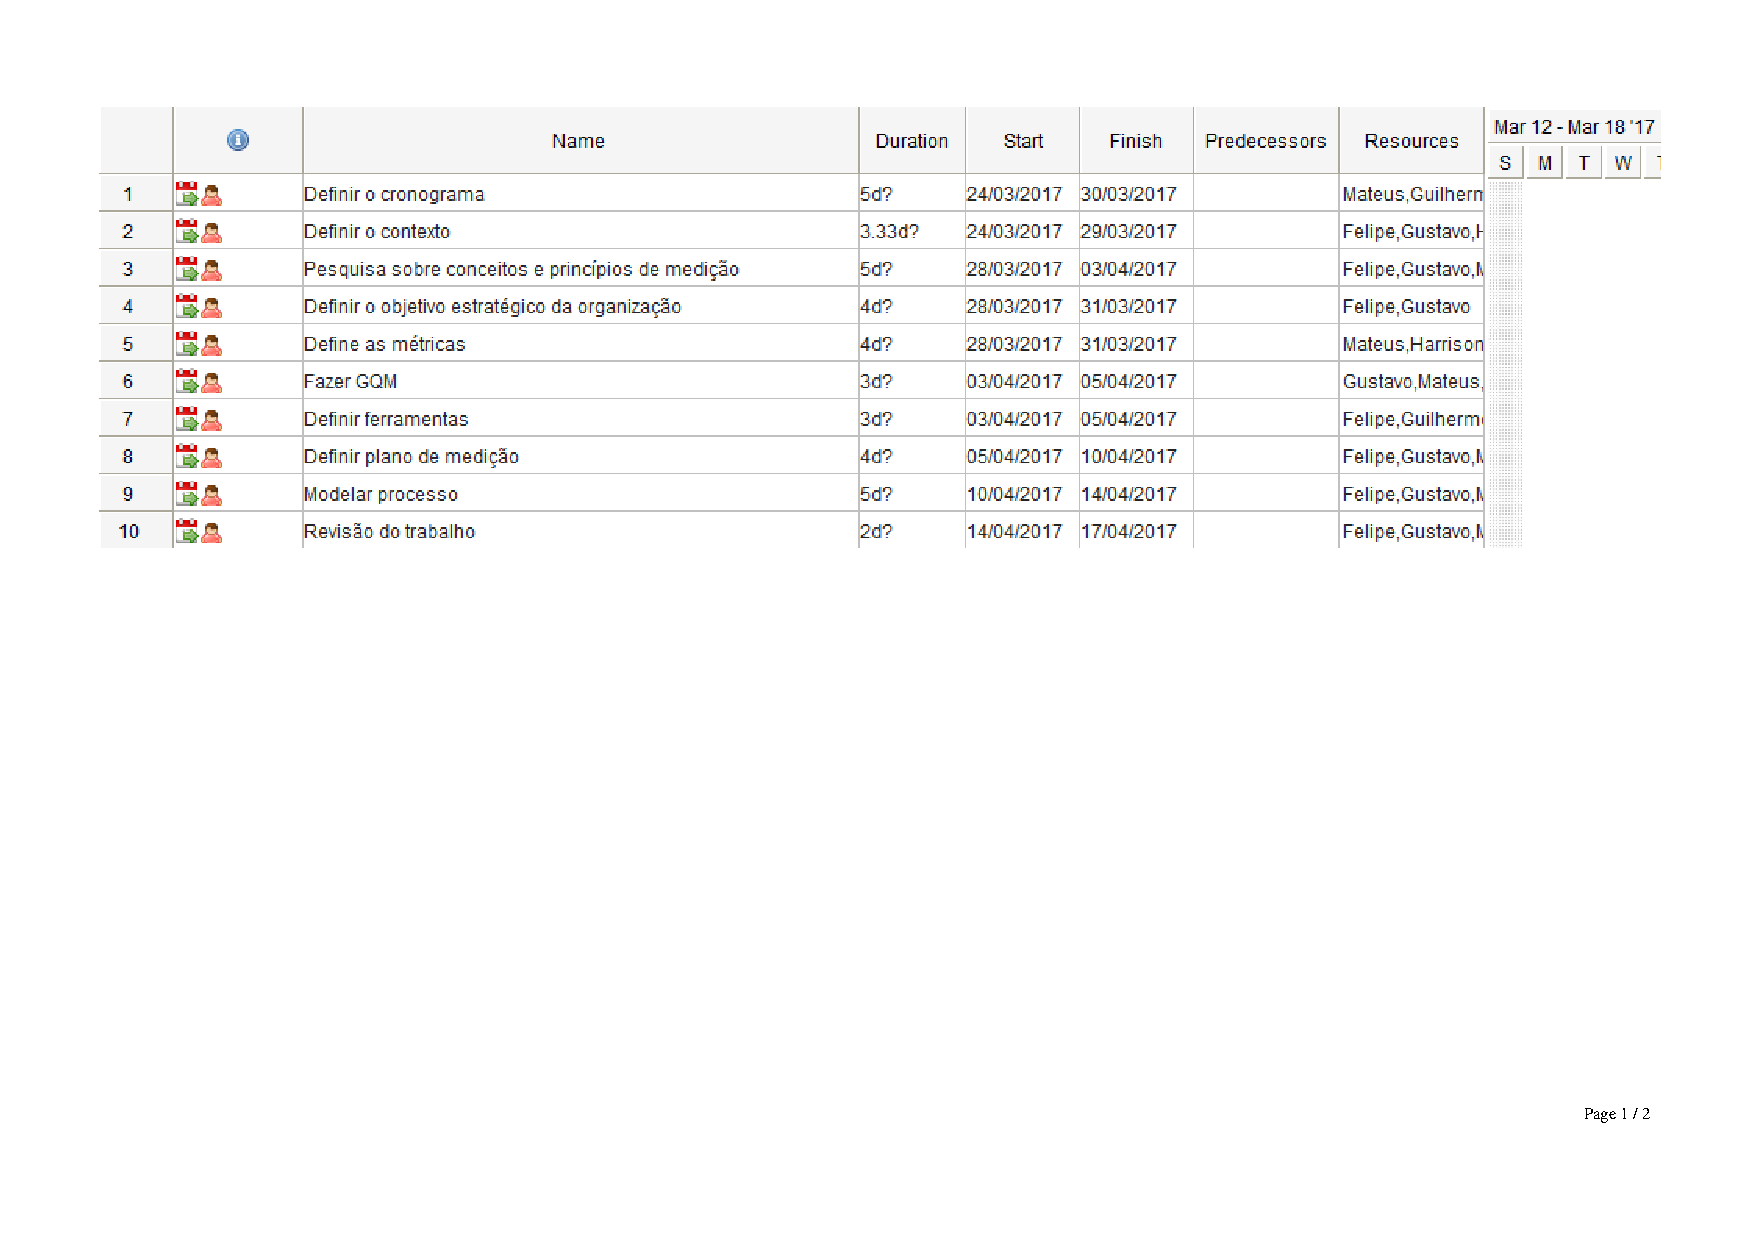
\includegraphics [scale=0.35]{figuras/processo/cronograma}
		\caption{Cronograma utilizado pela equipe}
	\end{figure}
	\newpage
\section{Descrição das Atividades}

Nessa seção serão descritas a atividades elustradas no processo no capítulo 4 deste relatório, separando cada atividade de acordo com as fases relatadas na ISO/IEC/IEEE 15939:2008, descrevendo e indicando os responsáveis sobre as mesmas.

\subsection{Fase 1 - Estabelecer e manter compromisso com o processo de medição}
	\begin{tabular}{ |p{4cm}|p{6cm}| p{3cm} |}
	 \hline
	 Atividade 		& 		Descrição & Responsáveis \\
	 \hline
	 	Definir Escopo & Consiste em definir qual a unidade organizacional que a medição será aplicada &  Equipe de medição, equipe de desenvolvimento \\
	 \hline
	 	Definir papéis & Consiste em definir recursos, responsabilidades e atribuir os recursos as pessoas que possuem a competência necessária para exercer a função & Equipe de medição \\
	 \hline
	\end{tabular}


\subsection{Fase 2 - Planejar o processo de medição}

	\begin{tabular}{ |p{4cm}|p{6cm}| p{3cm} |}
	 \hline
	 Atividade 		& 		Descrição & Responsáveis \\
	 \hline
	 	Caracterizar unidade organizacional & Consiste em caracterizar a unidade organizacional e o que eles almejam de forma que seja possível montar um modelo GQM &  Equipe de medição, equipe de desenvolvimento \\
	 \hline
	 	Identificar necessidades de informação & Consiste em identificar e priorizar quais são os objetivos da medição de forma que afete o processo de desenvolvimento da equipe &  Equipe de medição \\
	 \hline
	 	Levantar questões sobre os objetivos & Consiste no levantamento de questões de forma que caracterize como os objetivos serão alcançados &  Equipe de medição \\
	 \hline
	 Levantar métricas para as questões & Consiste em definir quais as métricas a serem avaliadas, de forma que as questões definidas sejam respondidas, além de auxiliarem na criação dos indicadores &  Equipe de medição \\
	 \hline
	 Validar GQM & Essa atividade consiste em verificar se todos objetivos, questões e métricas atendem às necessidades dos stakeholders &  Equipe de medição \\
	 \hline
	 Definir tecnologias de apoio & Inclui a verificação e definição de ferramentas que auxiliem na coleta das métricas &  Equipe de medição \\
	 \hline
	\end{tabular}

\subsection{Fase 3 - Executar o processo de medição}

	\begin{tabular}{ |p{4cm}|p{6cm}| p{3cm} |}
	 \hline
	 Atividade 		& 		Descrição & Responsáveis \\
	 \hline
	 	Integrar processo de medição no desenvolvimento & Configurar ferramentas e atividades junto com a equipe de desenvolvimento, para a coleta de métricas &  Equipe de medição \\
	 \hline
	 	Coletar Dados & Coletar as métricas por meio das ferramentas e métodos estabelecidos no plano de medição, e armazená-las para efetuar análise &  Equipe de medição, equipe de desenvolvimento \\
	 \hline
	 	Analisar os Dados & Analisar as métricas coletadas para que se possa retirar informações úteis que auxilirão a equipe de desenvolvimento &  Equipe de medição \\
	 \hline
	 	Comunicar resultados & Produzir um documento que explique de forma objetiva as informações derivadas das métricas para a equipe de desenvolvimento &  Equipe de medição \\
	 \hline
	\end{tabular}

\subsection{Fase 4 - Avaliar o processo de medição}

	\begin{tabular}{ |p{4cm}|p{6cm}| p{3cm} |}

	 \hline
	 Atividade 		& 		Descrição & Responsáveis \\
	 \hline
	 	Avaliar o processo de execução & Consiste em verificar os pontos fortes e fracos no processo utilizado pela equipe de desenvolvimento ao decorrer do projeto &  Equipe de medição \\
	 \hline
	 	Comunicar melhorias propostas & A equipe de medição dará um feedback aos stakeholders sobre possíveis melhorias, de forma que eles possam aprovar ou não tais propostas &  Equipe de medição, equipe de desenvolvimento \\
	 \hline

	\end{tabular}
